\chapter[LDoctor: Hybrid Analysis Routines for Inefficient Loops]{LDoctor: Hybrid Analysis Routines for Inefficient Loops}
\label{chap:ldoctor}

Statistical performance debugging discussed in the last chapter can 
identify which loop is the root cause for a performance problem. 
However, it cannot provide detailed root-cause information, 
such as why a loop is inefficient and how developers might fix the problem. 

In this chapter, we first conduct an empirical study to understand what are
fine-grained root-cause information for inefficient loops in the real world. 
We then design a series of static-dynamic hybrid analysis routines that can
help identify accurate fine-grained root-cause information for inefficient loops.
We further use sampling techniques to lower our diagnosis overhead without
hurting diagnosis accuracy or latency. Evaluation using real-world inefficient loops 
shows that our tool can provide good coverage and accuracy, 
with small runtime overhead.

\section{Introduction}
\label{sec:6_intro}
\subsection{Motivation}

In Chapter~\ref{chap:sd}, 
we discussed how to apply statistical debugging to performance failure diagnosis. 
Given the symptom of 
a performance problem (e.g., two similar inputs leading to very
different execution speed),
statistical debugging, an approach widely used for diagnosing
functional failures~\citep{liblit03,liblit05,tarantula1}, can
accurately identify control-flow constructs that are most correlated with
the performance problem by comparing problematic runs and regular runs.
Unfortunately, for loop-related 
performance problems, which contribute to two thirds of user-reported
real-world performance problems studied in Chapter~\ref{chap:sd},
statistical debugging is not very effective.
Although it can identify the root-cause loop, it does not provide any 
information regarding why the loop is inefficient and hence is not very helpful
in fixing the performance problem.

Figure~\ref{fig:GCC27733} shows a real-world performance bug in GCC. 
Function \texttt{synth\_mult} is used to compute the best algorithm for 
multiplying \texttt{t}. It is so time consuming that developers tried 
speeding it up through memoization ---
hash-table
\texttt{alg\_hash} is used to remember which \texttt{t} has been processed
in the past and what is the processing result. 
Unfortunately, a small mistake in the type declaration of hash-table
entry \texttt{alg\_hash\_entry} causes memoization not to work when \texttt{t}
is larger than the maximum value type-\texttt{int} can represent.
As a result, under certain workload, \texttt{synth\_mult} conducts a lot of
redundant computation for same \texttt{t} values recursively, leading to
huge performance problems.  In practice, developers know the problem is inside
\texttt{synth\_mult} very early. However, since this function is 
complicated, it took them several weeks to figure out the root cause. 
If a tool can tell them not only which loop\footnote{Recursive functions are
handled similarly as loops in this chapter.}
is the root cause but also why the loop is inefficient (i.e., lot of redundant
computation and the need for better memoization in this example), 
the diagnosis and bug fixing
process would be much easier for developers. 

Clearly, more research is needed to improve the state of the art of performance
diagnosis. Diagnosis techniques that can provide fine-grained root-cause information for common performance problems,
especially loop-related performance problems, is well desired.

\subsection{Contributions}
This chapter presents a tool, \Tool, that can effectively provide fine-grained root causes for inefficient loops. 

\Tool targets the most common type of performance problems, 
inefficient loops, according to
empirical studies in Chapter~\ref{chap:study} and Chapter~\ref{chap:sd}.
\Tool also targets a challenging problem. Although
statistical debugging (Chapter~\ref{chap:sd})
can help identify suspicious loops that are highly correlated with 
user-perceived performance problems,
it provides no information about why the suspicious loop is inefficient,
not to mention providing fix suggestions. Although various
bug-detection techniques \citep{Cachetor,Alabama,CARAMEL} can help detect
loop-related performance bugs, they all suffer from generality problems,
covering only a specific type of loop problems each; the dynamic
tools \citep{Cachetor,Alabama} also suffer from performance
problem, imposing 10X slowdown or more.

\Tool can provide good coverage, accuracy and performance simultaneously:
1) Coverage. \Tool can cover most common root causes for inefficient loops. 
2) Accuracy. \Tool can accurately point out whether a loop is inefficient, explain why the loop is inefficient, 
and provide correct fix suggestions. 
3) Performance. \Tool incurs a low runtime overhead.

We build \Tool through the following three steps.

First, figuring out a taxonomy for the root causes of common inefficient loops.
Such a taxonomy is the prerequisite to developing a general and accurate
diagnosis tool. Guided by a thorough study of 45 real-world inefficient loop problems, we come up with a hierarchical root-cause taxonomy for
inefficient loops. 
Our empirical study shows that our taxonomy is general enough to cover
common inefficient loops, and also specific enough to help developers understand
and fix the performance problem. We will present more details 
in Section~\ref{sec:6_study}.

Second, building a tool(kit) \Tool that can automatically and accurately
identify the fine-grained root-cause type of a suspicious loop 
and provide fix-strategy suggestions. 
We achieve this following several principles:

\begin{itemize}
\item Focused checking. 
Different from performance-bug detection tools that blindly check the whole
software, \Tool focuses on performance symptoms and only check inefficient
loop candidates identified by existing tools, a statistical debugging
tool (Chapter~\ref{chap:sd}) in our current prototype. 
This focused study is crucial for \Tool to achieve high
accuracy.

\item Root-cause taxonomy guided design. To provide the needed coverage, we follow
the root-cause taxonomy discussed above and design analysis routines for 
every root-cause sub-category. Given a candidate inefficient loop, we will 
apply a series of analysis to it to see if it matches any type of inefficiency.

\item Static-dynamic hybrid analysis to balance performance and accuracy.
As we will see, static analysis alone cannot accurately identify 
inefficiency root causes, especially because some inefficiency problems only
happen under specific workload. However, pure dynamic analysis will 
cause too large 
runtime overhead. Therefore, we take a hybrid approach to achieve both
performance and accuracy goals.
\end{itemize}

Third, using sampling to further lower the runtime overhead of \Tool, without
degrading diagnosis capability. Random sampling is a natural fit for performance
diagnosis due to the repetitive nature of inefficient codes, especially
inefficient loops.

We have evaluated \Tool on 18 real-world performance problems. 
Evaluation results show that \Tool can accurately identify the detailed
root cause for all benchmarks and provide correct fix-strategy suggestion for
16 benchmarks. All these are achieved with low runtime overhead.

 

\section{Root-Cause Taxonomy}
\label{sec:study}

The first task we are facing is to figure out a root-cause taxonomy for
real-world inefficient loops. 
Our taxonomy design is guided by checking a benchmark suite of real-world
inefficient loops, collected by previous work \citep{SongOOPSLA2014,PerfBug}. 
We also try to satisfy three requirements in our design.
(1) Coverage: covering
a big portion of real-world inefficient loop problems; 
(2) Actionability: each root-cause category should be informative enough 
to help developers
decide how to fix a performance problem; 
(3) Generality: too application-specific root causes will not work, as we
need to build diagnosis tools to automatically identify these root causes 
without developers' help.
In this section, we will first present our taxonomy, together with real-world
examples, followed by our empirical study about how a suite of real-world 
inefficient
loop problems fall into our root-cause categories.

We should note that we are definitely not the first one who tries to categorize
the root-cause patterns of performance problems. We are also not the first
to identify many of the root-cause categories below. Instead, guided by
previous work and our empirical study, we try to figure out our own taxonomy 
that satisfy the above three requirements and can
work well with the diagnosis tool that we will build later.

\subsection{Taxonomy}
\label{sec:study_tax}
Our taxonomy contains two major root cause categories,
\textit{resultless} and \textit{redundancy}, and several sub-categories, 
as below.

\underline{\textit{\textbf{Resultless}}}
Resultless loops spend a lot of time in computation that does not 
produce any results that will be used after the loop.
Depending on when such resultless computation is conducted, we further
consider four sub-categories.

{\textbf{0*}}: 
This type of loops never produce any results in any iteration.
This type of loops should be rare in mature software systems.
They should simply be deleted from the program.
%Question: dynamic or static?

\begin{figure}
\codefig{Mozilla347306}
\caption{A resultless 0*1? bug in Mozilla}
\label{fig:Mozilla347306}
\end{figure}


%\begin{figure}[h]
%\centering
%\lstset{basicstyle=\ttfamily\fontsize{8}{8}\selectfont,
%     morekeywords={+},keepspaces=true}
%  \mbox{\lstinputlisting[mathescape,boxpos=t]{figures/Mozilla347306.c}}
%\caption{A resultless 0*1? bug in Mozilla}
%\label{fig:Mozilla347306}
%\end{figure}

{\textbf{0*1?}}:
This type of loops only produce results in the last iteration, if any. 
They are often related to search: they check a sequence of elements one
by one until the right one is found.
Not all loops of this type are inefficient. If they are, they are often
fixed by data-structure changes.
Figure~\ref{fig:Mozilla347306} shows an example from Mozilla
JavaScript engine. 
The loop searches through an array containing source code information for the input \texttt{pc}. 
In practice, this loop needs to execute more than 10000 iterations for 
many long JavaScript encountered by users, which leads to huge 
performance problems --- web browsers freeze. To fix this problem, 
developers simply replace array with hash table when processing long
JavaScript files.
% This improve the performance by 52.60{\bf X}.

%\comment{
%This loop searches through xxx for xxx.
%When xx, this loop often needs to execute xx iterations, which is very
%time consuming.
%The developers simply change the data-structure of xx from xx to a hash
%table, which eliminates this loop and improving the performance by xxx.}
%%Linhai, you have to describe examples using words people can understand
%%and you have to provide useful information, such as what is the purpose
%% of the loop. What is the loop searching for? What is the bug-triggering
%%workload; how bad the performance (throughput or latency) was; how good
%%is the fixed version in terms of performance.
%\comment{
%\textcolor{red}{
%MySQL\#27287 is caused by linear backward searching for parent node during XML string parsing. 
%In each iteration of the buggy loop, one previous sibling will be skipped, 
%and in the last iteration, parent node will be returned. 
%The patch applies a stack-like data structure to keep all parent nodes who have unparsed children to avoid the linear backward searching.
%} } 
%Linhai, I have no idea what you are talking about here for mysql27287

%TOADD: performance diagnosis is different from bug detection%
%in many cases, there is no absolutely ``bad'' cases. performance problems are
%often a trade-off between code simplicity, performance, xxx.
%treating it like bug detection will inevitably lead to false positives
%we are providing information to developers



\begin{figure}
\codefig{GCC46401}
\caption{A resultless [0$|$1]* bug in GCC}
\label{fig:GCC46401}
\end{figure}

%\begin{figure}[h]
%\centering
%\lstset{basicstyle=\ttfamily\fontsize{8}{8}\selectfont,
%     morekeywords={+},keepspaces=true}
%  \mbox{\lstinputlisting[mathescape,boxpos=t]{figures/GCC46401.c}}
%\caption{A resultless [0$|$1]* bug in GCC }
%\label{fig:GCC46401}
%\end{figure}


{\textbf{[0$|$1]*}}:
Every iteration in this type of loops may or may not produce results.
Under certain workload, the majority of the loop iterations do not produce
any results and lead to performance problems perceived by end users.
The inefficiency problem caused by this type of loops can often be solved
by adding extra conditions to skip the loop under certain contexts.
Figure~\ref{fig:GCC46401} shows such an example from GCC.
%how users perceive this problem
%explain how every iteration may or may not produce any results
%explain the fix
Only when the if branch executed,
one iteration will generate results. 
The bug happens when GCC checks violation of sequence point rule. 
The user notice severe performance degradation when enabling the checking. 
The buggy loop is super-linear inefficient in terms of the number of operands
in one expression. The buggy input contains an expression, which is long and special. 
The loop takes a lot of iterations during bad run, but none of the iterations will 
generate results. 
The patch is to add extra checking before processing each operand. When it also has
the special feature like the bad input, the loop will be skipped. 



{\textbf{[1]*}}:
Loops in this category always generate results in almost all iterations. 
They are inefficient, because the results generated could be useless due to
some high-level semantic reasons.
Understanding and fixing this type of inefficiency problems often require
deep understanding of the program and are difficult to automate.
For example, several Mozilla performance problems are caused by 
loops that contain intensive GUI operations.
Although every iteration of these loops produce side effects, 
the performance problem forced developers to change the program 
and batch/skip some GUI operations.


\begin{figure}
\codefig{Mozilla477564}
\caption{A cross-loop redundant bug in Mozilla}
\label{fig:Mozilla477564}
\end{figure}

%\begin{figure}[h]
%\centering
%\lstset{basicstyle=\ttfamily\fontsize{8}{8}\selectfont,
%     morekeywords={+},keepspaces=true}
%  \mbox{\lstinputlisting[mathescape,boxpos=t]{figures/Mozilla477564.js}}
%\caption{A cross-loop redundant bug in Mozilla }
%\label{fig:Mozilla477564}
%\end{figure}

\underline{\textit{\textbf{Redundant}}}
Redundant loops spend a lot of time in repeating computation that is already
conducted.
Depending on the unit of the redundant computation, we further consider 
two sub-categories.

%\begin{figure}[h]
%\centering
%\lstset{basicstyle=\ttfamily\fontsize{8}{8}\selectfont,
%     morekeywords={+},keepspaces=true}
%  \mbox{\lstinputlisting[mathescape,boxpos=t]{figures/GCC1687.c}}
%\caption{A cross-iteration redundant bug in GCC 
% (\texttt{walk\_tree} will call itself recursively inside the loop, 
% and during buggy run, many iterations are doing exactly the same thing.)  }
%\label{fig:GCC1687}
%\end{figure}

\begin{figure}
\codefig{Mozilla490742}
\caption{A cross-iteration redundant bug in Mozilla}
\label{fig:Mozilla490742}
\end{figure}


%\begin{figure}[h]
%\centering
%\lstset{basicstyle=\ttfamily\fontsize{8}{8}\selectfont,
%     morekeywords={+},keepspaces=true}
%  \mbox{\lstinputlisting[mathescape,boxpos=t]{figures/Mozilla490742.js}}
%\caption{A cross-iteration redundant bug in Mozilla }
%\label{fig:Mozilla490742}
%\end{figure}

{\textbf{Cross-iteration Redundancy}}:
Loop iteration is the redundancy unit here:
one iteration repeats
repeating what was already done by an earlier iteration of the same loop.
Here, we consider recursive function calls as a loop, treating one function 
call instance as one loop iteration. 
This type of inefficiency is often fixed by memoization or batching, depending
on whether the redundancy involves I/O operations.
For example, GCC\#27733 shown in Figure~\ref{fig:GCC27733} 
is fixed by better memoization. 
%Another bug similar to GCC\#27733 is shown in Figure~\ref{fig:GCC1687}. 
%This bug is fixed by using a hash table to avoid visiting the same sub-tree twice.
Mozilla\#490742 in Figure~\ref{fig:Mozilla490742} represents a slightly different type of cross-iteration
redundancy. The inefficient loop in this case saves one URL into the ``Favorite
Links'' database in each iteration. One database transaction in each iteration
turns out to be to time consuming, with too much redundant work across
iterations. At the end, developers decide to batch all database updates into 
one big transaction, which speeds up some workload like 
bookmarking 50 tabs 
from popping up timeout windows to not blocking.
%xxx from several minutes
%to a couple of seconds.

{\textbf{Cross-loop Redundancy}}:
A whole loop is the redundancy unit here:
one dynamic instance of a loop spends a big chunk, if not all, of its
computation in repeating the work already done by an
earlier instance of the same loop.
Developers often fix this type of inefficiency problems through memoization:
caching the earlier computation results and skip following redundant loops.
Mozilla\#477564 shown in Figure~\ref{fig:Mozilla477564} is an example for this type of bugs. 
The buggy loop is to count how many previous siblings of the input \texttt{aNode} have the same name and URI. 
There is an outer loop for the buggy one, and the outer loop will update \texttt{aNode} by using its next siblings. 
The bug is fixed by saving the calculated count for each node. 
A new count value is calculated by adding one to the saved count value of the nearest previous sibling with the same name and URI.


\subsection{Empirical study}
\label{sec:tax_study}
Having presented our taxonomy above, we will see how it works for a set of
real-world inefficient loop problems collected by previous work
\citep{SongOOPSLA2014,PerfBug}. Specifically, we want to check the 
coverage and the actionability of our taxonomy presented above:
(1) How common are real-world performance problems caused by the 
patterns discussed above?
(2) How are real-world problems fixed by developers? Can we predict their
fix strategies based on the root-cause pattern?

\subsubsection{Methodology}
\begin{table}[h!]
\scriptsize
\centering
\begin{tabular}{@{\hspace{3pt}}l@{\hspace{3pt}}@{\hspace{3pt}}c@{\hspace{3pt}}}
\toprule
Application Suite Description (language) & \# Bugs \\
\midrule                            
{\bf Apache Suite} 	 & 11\\
%\cline{1-1}
{HTTPD:	Web Server (C)	}& \\
{TomCat:  Web Application Server (Java)}& \\
{Ant:	Build management utility (Java)}& \\
%\hline
%JMeter	& Load test utility (Java) & \\
\midrule                            
{\bf Chromium Suite} Google Chrome browser (C/C++) & 4\\
\midrule
%\multicolumn{2}{|l|}
{\bf GCC Suite}  GCC \& G++ Compiler (C/C++)     & 8\\
\midrule
{\bf Mozilla Suite}  & 12\\
%\cline{1-1}
{Firefox: Web Browser (C++, JavaScript)}& 	\\
{Thunderbird: Email Client (C++, JavaScript)}& \\
\midrule
{\bf MySQL Suite}     & 10	\\
%\cline{1-1}
{Server: Database Server (C/C++)}&  	\\
%\cline{1}
{Connector: DB Client Libraries (C/C++/Java/.Net)} &  	\\
\midrule
{\bf Total}	   & 45 \\
\bottomrule
\end{tabular}
\caption{Applications and bugs used in the study}
\label{tab:app_bug}
\end{table}

Previous work \citep{PerfBug,SongOOPSLA2014} studied the on-line bug
databases of five representative open-source software projects, as 
shown in Table \ref{tab:app_bug}. Through a mix of random sampling and 
manual inspection, they 
found 65 performance problems that are perceived and reported by users. 
Among these 65 problems, 45 problems are related to inefficient loops and 
hence are the target of the study 
here\footnote{The definition of ``loop-related'' in this paper is a little
bit broader than earlier paper~\citep{SongOOPSLA2014}, which only considers
43 problems as loop-related. }.
More details can be found in the original papers that collect
these bugs. 

\subsubsection{Observations}
\label{sec:study_ob}
\begin{table*}[tb!]
\begin{adjustwidth}{-.5in}{-.5in}
\scriptsize
\centering
{
\begin{tabular}{lccccccl}
\toprule
&Apache&Chrome&GCC&Mozilla&MySQL&Total&Fix Strategy\\
\midrule
Total \# of loop-related bugs & 11 & 4 & 8 & 12 & 10 & 45 &  \\
\midrule
\multicolumn{8}{c}{\# of {\textit {Resultless}} bugs}\\
\multicolumn{1}{l}{ {\bf 0*} }
&0&0&0&0&0&0&\\
\multicolumn{1}{l}{ {\bf 0*1?} }
&0&0&0&2&3&5&C(4)$|$S(1)\\
\multicolumn{1}{l}{{\bf [0$|$1]*}}
&0&1&1&1&1&4&S(4)\\
\multicolumn{1}{l}{{\bf 1*}}
&1&2&3&6&3&15& B(4)$|$S(4)$|$O(7)\\
%&0&2&0&5&0&7&B(4)$|$S(3)\\
%&1&0&3&1&3&8&\\
\midrule
\multicolumn{8}{c}{ \# of {\textit {Redundant}} bugs}\\
\multicolumn{1}{l}{Cross-{\bf iteration} redundancy}
&7&1&2&1&1&12&B(4)$|$M(7)$|$O(1)\\
\multicolumn{1}{l}{ Cross-{\bf loop} redundancy}
&3&0&2&2&2&9&B(4)$|$M(5)\\
  %MySQL15811 is moved from 1* to here; consider it as fixed by M
%\hline
%\multicolumn{8}{|c|}{ \# of {\textit {Other}} bugs}\\
%\multicolumn{1}{|l}{Not in above categories}
\bottomrule
\end{tabular}
}
\end{adjustwidth}
\caption{Number of bugs in each root-cause category. 
B, M, S, C, and O represent different fix strategies:
B(atching),  
M(emoization), 
S(kipping the loop),
C(hange the data structure), and O(thers). The numbers in the 
parentheses denote the number of problems that are fixed using specific
fix strategies.}
\label{tab:root}
\end{table*}



\underline{Are the root-causes in our taxonomy common?}
The answer is \textit{yes}.
Resultless loops are about as common as redundant loops
(24 vs. 21).
Intuitively, 0* loops, where no iteration produces any results,
are rare in mature software. In fact, no bugs in this
benchmark suite belong to this category.
All other root-cause sub-categories are well represented.


\underline{How are real-world performance bugs fixed?}
Overall, the fix strategies are well aligned with root-cause patterns.
For example, 
all inefficient loops with resultless [0$|$1]* are
fixed by skipping the loop under certain contexts,
and almost all inefficient loops with redundant root causes are fixed either by 
memoization or batching the computation. 
In fact, as we will discuss later, simple analysis can tell whether 
memoization or batching should be used to fix a problem.
The only problem is that there are no silver bullets for 1* loops.
%all inefficient loops with xx root cause are fixed by xxx.
%xxx

\paragraph{Implications}
As we can see, resultless loops and redundant loops are both common reasons
that cause user-perceived performance problems in practice. The root-cause
categories discussed above also match with developers' fix strategy well ---
with a little bit amount of extra analysis, one can pretty much predict the fix strategy based on the root-cause pattern.
Consequently, tools that cover these root causes will have high
chances to satisfy the coverage and accuracy requirements of performance 
diagnosis.

%TODO even for the other, there are things we could do ...

\subsubsection{Caveats} 
Just as previous empirical study work, 
our empirical study above needs to be interpreted with our methodology in mind. 
The performance bugs examined above cover a variety of applications, workload, 
development environments and programming languages. 
However, there are still uncovered cases, like distributed systems, 
and scientific computation. 

Previous work~\citep{PerfBug, SongOOPSLA2014} uses developers tagging and
on-line developer/user discussion to judge whether a bug report is about
performance problems and whether 
the performance problem under discussion is noticed and reported by users
or not.
We follow the methodology used in previous work~\citep{SongOOPSLA2014} to judge 
whether the root-cause of a performance problem is related to loops or not.
We do not intentionally ignore any aspect of loop-related performance problems. 
Some loop-related performance problems may never be noticed by end users
or never be fixed by developers, and hence skip our study. However,
there are no conceivable ways to study them. 

We believe that the bugs in our study provide a representative sample of the 
well-documented and
fixed performance bugs that are user-perceived and loop-related in the studied 
applications. 
Since we did not set up the root-cause taxonomy to fit particular
bugs in this bug benchmark suite, we believe our taxonomy and diagnosis
framework presented below will go beyond these sampled performance bugs. 


\section{\Tool design}
\label{sec:6_design}
\Tool is composed of a series of analysis routines, each designed to 
identify whether a given loop belongs to one specific type of root causes,
as we will present below. 

As briefly mentioned in Section \ref{sec:6_intro}, the design of these analysis routines follows the following principles.
\begin{itemize}
\item Providing diagnosis information, not detecting bugs. \Tool will be  
used together with other performance diagnosis tools (Chapter~\ref{chap:sd})
and focus on a small
number of loops that are most correlated with a specific performance symptom,
instead of being applied to the whole program. Therefore, we will have different
design trade-offs in terms of coverage and accuracy, comparing with 
bug detection tools.

\item Static-dynamic hybrid analysis. As we will see, static analysis alone
will not be able to provide all the needed information for performance
diagnosis; dynamic analysis alone will incur too much unnecessary overhead.
Therefore, we will use static-dynamic hybrid approach throughout our design.

\item Using sampling to decrease runtime overhead. Loop-related 
performance problems have the unique nature of repetitiveness, which make 
them a natural fit for random sampling. Therefore, we will design different
sampling schemes for different analysis routines.
\end{itemize}

\subsection{Resultless Checker}
\label{sec:6_workless}

Our resultless checker includes two parts. First, we use static analysis
to figure out which are the side-effect instructions in a loop and hence
decide whether a loop belongs to 0*, 0*1?, [0$|$1]*, or 1*. Second, for
0*1? and [0$|$1]* loops, we use
dynamic analysis to figure out what portion of loop iterations are
resultless at run time, which will help decide whether the loop is indeed
inefficient.

%\begin{figure}[ht]
%\center
%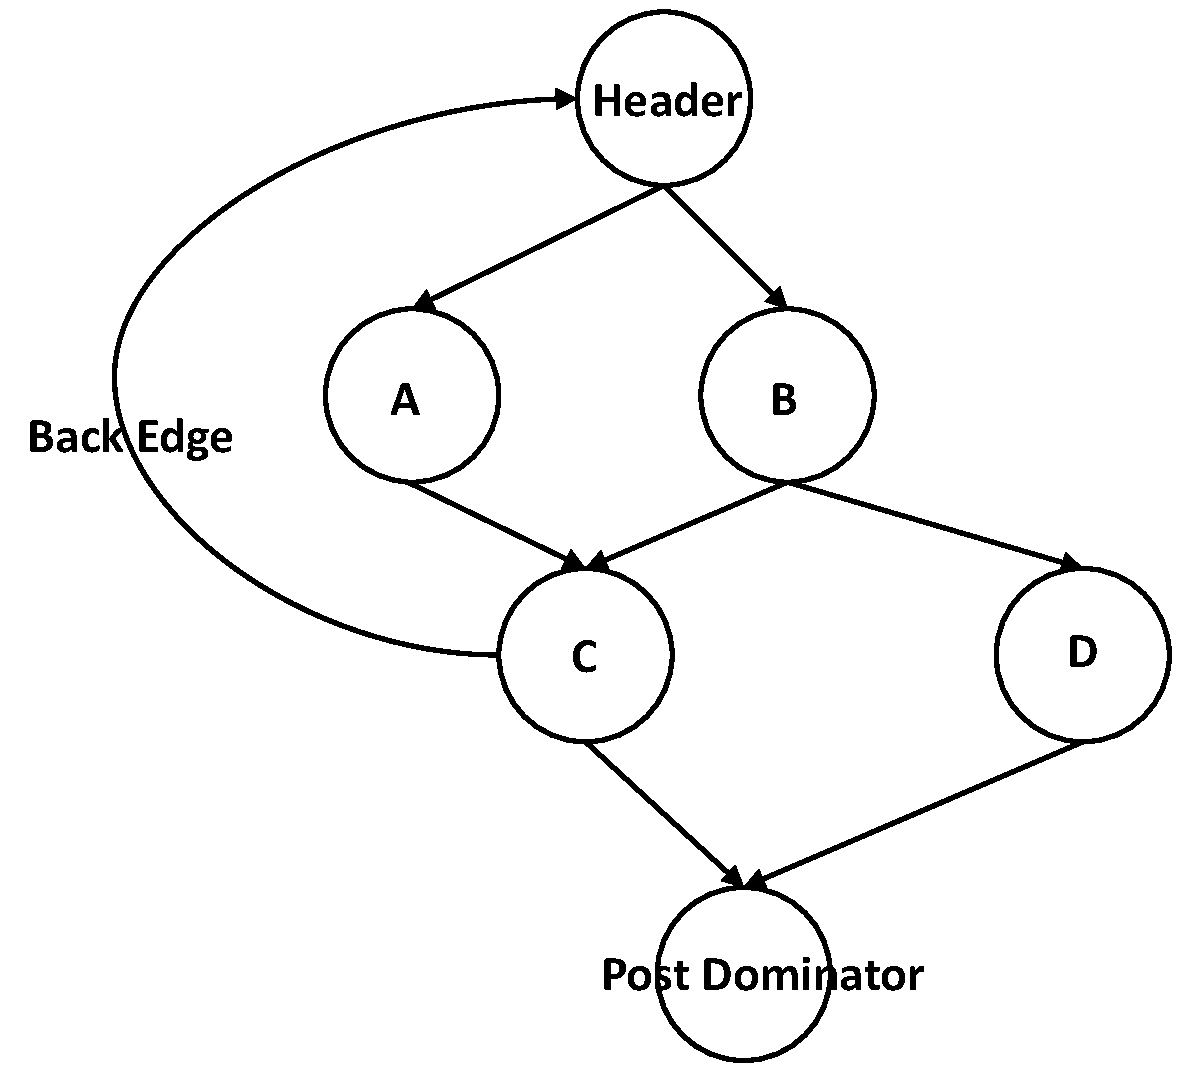
\includegraphics[width=0.7\linewidth]{figures/workless.pdf}
%\caption{Examples for different types of basic blocks inside a loop}
%\label{fig:block_type}
%\end{figure}

\subsubsection{Static Analysis}
\label{sec:6_s_workless}

We consider side-effect instructions as those instructions that write to
variables defined outside the loop. The analysis to identify side-effect
instructions is straightforward. We consider all functions that are called
by a loop directly or indirectly --- a function $F$ that updates variables
defined outside $F$ makes the corresponding call statement in $F$'s
caller a side-effect instruction.
We consider all library functions or function calls through function pointers 
as functions that have side effects, 
unless the library functions are specially marked by us in a white list.

After identifying side-effect instructions, it is straight-forward to
categorize loops into the four types discussed above.
Loop 0* contains no side-effect instructions. 
Loop 1* contains at least one side-effect instruction along every path that
starts from the loop header and ends at the loop header.
The remaining cases are either 
0*1? or [0$|$1]*. 
Differentiating these two cases is also straight-forward.
In short, when the basic block that contains side-effect instructions
is part of the natural loop, the case
belongs to [0$|$1]*; instead, if the side-effect basic block is strictly post-dominated
by one of the loop-exit blocks and is dominated by the loop header, yet is
not part of the natural loop, the case belongs to 0*1?.

Finally, since the 1* pattern contains the least amount of information
about computation \textit{inefficiency}, \Tool will not report a loop's
root-cause type as 1*, if more informative root-cause type is identified 
for this loop (e.g., cross-iteration or cross-loop redundancy).

%TODO Shan will rewrite the next two paragraphs
\subsubsection{Dynamic Monitoring}
\label{sec:6_d_workless}

Except for 0*, none of the other three type of loops are inefficient for sure.
We need dynamic analysis to figure out what portion of loop iterations are
resultless at run time, which will help decide whether the loop is indeed
the root cause of a user-perceived performance problem and worth fixing.

For a 0*1? loop, since it only generates results in the last iteration, we 
only need to know the total number of iterations (or the average total number 
of iterations when the loop has multiple instances) to figure out the 
\textit{resultless rate} of the loop. The implementation is straightforward
--- we initialize a local counter to be 0 in the pre-header of the loop; we 
increase the counter by 1 in the loop header to count the number of 
iterations; 
we dump that local counter value to a global counter when the loop exits.

For [0$|$1]*, we need to count not only the total number of iterations, but
also the exact number of iterations that execute side-effect instructions
at run time. 
To do that, our instrumentation uses a local boolean variable 
\texttt{HasResult} to represent whether one iteration have side effect or not. 
\texttt{HasResult} is set to \texttt{False} in the loop header, and set to
\texttt{True} after each side-effect instruction. It will be used to help
count the number of side-effect iterations. For performance concerns,
before instrumenting side-effect blocks, we check whether there are 
post-domination relation between each pair of side-effect blocks. 
If both block A and block B are side-effect blocks and block A post-dominates 
block B, we only instrument block A to update \texttt{HasResult}. 

We could speed up the above counting using sampling. However, since the 
runtime overhead of the above counting is low, as shown in Section 
\ref{sec:6_experiment}, our current prototype of \Tool does 
not use sampling for this part of runtime analysis.

%\subsubsection{Sampling}
%We calculate the average iteration number 
%and the ratio of working iteration based on a separated 
%process from on-line branch sampling discussed in~\cite{SongOOPSLA2014}.
%We need to instrument the buggy program and re-execute it by using bug-triggering input. 
%In the future, we could design an algorithm to calculate the two resultless metrics 
%based on branch sampling reports to get rid of the extra instrumentation and the extra bad run.   

\subsubsection{Limitations}
\label{sec:6_l_workless}
The technique designed in this section has the following limitations.
First, when callee may have side effect, we will consider it will have side effect in the caller side, 
and do not consider the real execution inside callee. This could bring false negatives, 
because we could miss resultless cases, 
where side effect instructions inside callee do not execute. 
Experiments results in Section~\ref{sec:6_experiment} show that this is not a big issue, 
since we do not miss any resultless bugs.  

Second, our dynamic instrumentation does not consider concurrent execution of the monitored loop, 
because most of buggy loops we study only execute in one single thread. 
When the monitored loop is executed in multi-thread, like loop marked with omp pragma, we need to synchronize updates to global variables. 

\subsection{Redundancy checker}
\label{sec:6_redundant}

\subsubsection{Design overview}
To check whether there is redundant computation across different iterations
of one loop instance or across different instances of one static loop, we need
to address several challenges.

\begin{figure}
\codefig{Apache34464}
\caption{A cross-loop redundant bug in Apache}
\label{fig:Apache34464}
\end{figure}



%\begin{figure}
%  \centering
%  \lstset{basicstyle=\ttfamily\fontsize{8}{8}\selectfont,
%     morekeywords={+},keepspaces=true}
%  \mbox{\lstinputlisting[mathescape,boxpos=t]{figures/Apache34464.c}}
%  \caption{A cross-loop redundant bug in Apache}
%  \label{fig:Apache34464}
%\end{figure}

\emph{How to judge redundancy between two iterations/loop-instances?}
Given two iterations (or loop-instances) $i_1$ and $i_2$, since they have 
the same source code, 
a naive, yet expensive, solution is to record and compare the return value of
every memory read conducted by $i_1$ and $i_2$. Two better alternative
solutions are to record and compare only the values written or read by the
side-effect instructions, such as 
line 10 in Figure~\ref{fig:Mozilla477564},
or the source instructions\footnote{We define source instructions in a code
region $r$ as a set of memory-read instructions that side-effect
instructions in $r$ depend on and do not depend on any other instructions
inside $r$.}, 
such as source[i] at line 11 of Figure~\ref{fig:Apache34464}.

Among the the above two potential solutions, our design chooses the second one.
The reason is that, if there is indeed
redundancy, repetitive patterns at the side-effect instructions are caused by
repetitive patterns in the source instructions.
For the purpose of performance diagnosis, it is
more informative to track the cause, rather than the effect.

\emph{How to handle partial redundancy?}
In practice, redundant loops may be doing largely the same, instead of exactly
the same, computation across iterations or loop instances. It is also possible
%TODO define loop instance.
that only some, instead of all, iterations in a loop are doing redundant
computation. We will discuss how we handle this issue in Section \ref{sec:6_cal}.



\emph{How to lower the overhead of record-and-compare?}
Even if we only record and compare the values returned by source instructions,
instead of all instructions in a loop, the runtime overhead and the log size
would still be large. We will use two ways to lower this time and spatial
overhead. First, static analysis can already tell some source instructions
will always return the same value across iterations/loop-instances, and hence
need not be traced at run time. Second, we can leverage the repetitive nature
of performance problems and use random sampling to lower the overhead without
degrading the diagnosis capability. We will discuss details of 
these two optimization in Section \ref{sec:6_inst} and \ref{sec:6_perf}.
%TODO static analysis alone is not sufficient, because some redundant is
%workload dependent

\emph{How to provide the most suitable fix-strategy suggestion?}
Finally, as discussed in Section \ref{sec:6_study_ob} and Table \ref{tab:6_root},
memoization and batching are both common fix strategies for redundant loops.
To pick the right fix strategies to fix a redundant loop, we will conduct 
some extra analysis. We will discuss this in Section \ref{sec:6_redundant_fix}.


\subsubsection{Identifying source instructions}
\label{sec:6_dependence}

Informally, we use static analysis to identify a set of 
memory-read instructions that the loop computation depends on. We refer
to these instructions as \textit{source} instructions. The values returned
from them at runtime will be tracked and compared to identify
redundant computation.

Specifically, we first identify side-effect instructions in the loop, as 
discussed in Section \ref{sec:6_s_workless}; we then conduct static slicing 
from these instructions, considering both control and data
dependency, to identify source instructions.

%TODO How do you handle constant values? I didn't get it.
Our slicing ends when it reaches either a local-variable read conducted
outside the loop or a heap/global-variable read anywhere in the program.
For the latter case, our slicing stops because tracking data-dependency
through heap/global variables is complicated in multi-threaded C/C++
programs. For the former case, 
not including local-variable reads inside the loop can help reduce the
amount of data that needs to be recorded. 
When there are function calls inside the loop,  
we conduct slicing for return values of callees and side-effect instructions
inside callees. 
%In order to reduce the number of memory read we need to record inside callees, 
%we calculate previous writes conducted to the same address for each local-structure read and local-array read. 
%Since local structures and local arrays are mainly used in the declared functions, 
%it is easy to know whether read or write conducted on them are applied to the same address. 
We omit encountered constant values through slicing, because constant values will not influence whether a loop or an iteration is redundant. 


%We conduct slicing to for return values of callees and side-effect instructions
%inside callees. In order to reduce the number of memory read we need to record, 
%we design a GEN-KILL based algorithm to analyze previous writes for read from local structures and arrays 
%inside callees.
%TODO Linhai, I have no idea what you are talking about below
%For a memory read inside a callee function, 
%if its source is a structure or an array declared in the same function, 
%we use a GEN-KILL based algorithm to analyze previous writes for these reads. 
%We do not track previous writes for other memory reads, because it is very difficult to do inter-procedural alias analysis.  

% function() {
%  struct A;
%  A.a = 10;     // place a,
%  if(...)
%  {
%     A.a = 20;  // place b, value defined in place a will be killed, and this place gen a new value
%     print A.a  // A.a will be 20, because only value defined in place a is live 
%  }
%  return A.a;  // there will be memory read here. 
%  //We will do analysis to track where is the previous write for field a of struct A.
%  //The result will be write in place a, and place b
%  //We then conduct dependence analysis for these two writes.
%  //We only do this for read from structure and array declared in the same function. 
% }

The analysis for cross-iteration and cross-loop redundancy analysis is pretty
much the same. The only difference is that, if a memory read instruction 
$i$ in a loop depends on the value returned by instruction $j$ in an earlier
iteration, we stop tracing the dependence at $i$ and consider $i$ as a
source instruction for cross-iteration redundancy analysis, while we continue
the slicing for cross-loop redundancy analysis. 
For example, 
the instruction defining the value of \texttt{i} is the only side-effect instruction 
for the loop at line 11 of Figure~\ref{fig:Apache34464}. 
The source instructions calculated by cross-loop dependence analysis include 
memory read \texttt{source[i]} inside the loop, 
and three values defined outside the loop, 
which represent the initial value of \texttt{i}, the value of \texttt{max} and \texttt{first} respectively. 
In contrast, 
the source instructions calculated by cross-iteration dependence analysis 
include value \texttt{i} defined in previous iteration, 
memory read \texttt{source[i]}, 
and two values defined outside the loop (\texttt{max} and \texttt{first}).  


\subsubsection{Identifying redundant loops}
\label{sec:6_cal}

After identifying source instructions, we instrument these source
instructions, so that the values returned by these memory read
instructions can be recorded at run time. Specifically, we will assign
a unique ID for each source instruction, and a pair of $<InstID, Value>$
will be recorded at run time with the execution of a source instruction.
Our trace also includes some delimiters and meta information that allows
trace analysis to differentiate values recorded from different loop
iterations, different loop instances, and so on.
%TODO
%All values defined outside the loop is recorded in block O. 
%We record a delimiter, loop instance number and values defined in previous iterations in block H1'.
%Since we only consider redundant iterations from the same loop instance,  
%we do not record values defined outside the loop for cross-iteration redundancy. 



After collecting values returned by source instructions from every iteration
of one or multiple loop instances, we need to process the trace and decide
whether the loops under study contain cross-iteration redundancy or 
cross-loop redundancy. We will first present our high-level algorithms, followed
by the exact implementation in our prototype.

\paragraph{High-level algorithms}
For cross-iteration redundancy, we need to answer two questions. 
First, how to judge whether
two iterations are doing redundant work --- should the two iterations conduct
exactly the same computation?
Second, is a (dynamic) loop problematic when it contains only few 
iterations that are
redundant with each other?

Our answer to these two questions stick to one principle: there should be
sufficient amount of redundant computation to make a loop likely root-cause
for a user-perceived performance problem and to make itself worthwhile to
get optimized by the developers. Consequently,
for the first question, \Tool takes a strict 
definition --- only iterations that are doing exactly the same computation are
considered redundant. Since one iterating may not contain too much computation,
a weaker definition here may lead to many false positives. For the 
second question, we believe there should be a threshold. In our current 
prototype,
when the number of distinct iterations is less than half of the total iterations, 
we consider the loop is cross-iteration redundant. 
%when the number of distinct iterations is less than half of the total iterations 
%iterations/(distinct iterations) = 2

\begin{figure}
\codefig{Apache37184}
\caption{A cross-iteration redundant bug in Apache}
\label{fig:Apache37184}
\end{figure}


%\begin{figure}
%  \centering
%  \lstset{basicstyle=\ttfamily\fontsize{8}{8}\selectfont,
%     morekeywords={+},keepspaces=true}
%  \mbox{\lstinputlisting[mathescape,boxpos=t]{figures/Apache37184.java}}
%  \caption{A cross-iteration redundant bug in Apache}
%  \label{fig:Apache37184}
%\end{figure}

For example, Figure~\ref{fig:Apache37184} shows a loop from Apache-Ant that
contains cross-iteration redundancy.
As we can see, under the problem triggering input, 
only several distinct listeners are contained inside the vector, and most of 
iterations of the loop inside function \texttt{fireMessageLoggedEvent}
are doing exactly the same computation. 
%The problem for this bug is that developers say that the performance 
%loss happens in fireMessageLoggedEvent, but in the code I found, function
%messageLogged does not contain anything, and it is an empty function.
%I guess either developers do not have correct understanding of this bug,
%or I did not find the correct codes. 





For cross-loop redundancy, we need to answer similar questions,
especially how to judge whether two loop instances are doing redundant work ---
should they contain exactly the same number of iterations and doing exactly
the same computation in each iteration?
%Second, is a (static) loop problematic when it contains two instances that
%are redundant with each other?

Our answers here are different from our answers above for cross-iteration
redundancy analysis.
We do not require two loop instances to
conduct exactly the same computation to be considered redundant. The rationale
is that a whole loop instance contains a lot of computation, much more than
one iteration in general. Even if only part of its computation
is redundant, it could still be the root-cause of a user-perceived performance
problem and worth developers' attention. 

In fact, in practice, we almost have never seen cases where different loop 
instances are doing exactly the same computation.
For example, Figure~\ref{fig:Mozilla477564} demonstrates a cross-loop redundancy
problem in Mozilla. Here, the
latter instances contain more iterations than previous instances. 
Figure~\ref{fig:Apache34464} shows an example in Apache, 
The inner loop, which starts from line 8,  
searches from the beginning of a string \texttt{sb} for a target sub-string 
\texttt{s}. Since the outer loop, which starts on line 30, appends one 
character to \texttt{sb} in every iteration, every inner loop instance is 
doing computation that is similar, but not exactly the same, 
from its previous instance.


\paragraph{Detailed algorithm implementation}

The implementation of checking cross-iteration redundancy is straightforward.
We will record a sequence of $<InstID, Value>$ pair for every monitored
iteration, with each $InstID$ representing a unique source instruction.
We consider two iterations to be redundant, if their sequences are exactly the
same. To make sure a loop contains sufficient redundant computation, 
we calculate a loop's \textit{cross-iteration redundancy rate} --- dividing 
the total number of iterations in the loop by the number of distinct iterations.
The smaller the rate is, with 1 being the minimum possible value, 
the less cross-iteration redundancy the loop contains.

The implementation of checking cross-loop redundancy goes through several
steps. First, for $k$ dynamic instances of a static loop $L$ that appear
at run time, denoted as $l_1$, $l_2$,
..., $l_k$, we check whether redundancy exists between $l_1$ and $l_2$, 
$l_2$ and $l_3$, and so on. Second, we compute a 
\textit{cross-loop redundancy rate} for $L$
--- dividing the number of redundant pairs by $k-1$.
The smaller the rate is, with 0 being the minimum possible value, the
less cross-loop redundancy $L$ contains.
Here we only check redundancy between consecutive loop instances, because  
checking the redundancy between every pairs of loop
instances would be very time consuming.

The key of this implementation is
to judge whether two dynamic loop instances $l_1$ and $l_2$ 
are redundant or not.
The challenge is that $l_1$ and $l_2$ may have executed different number of
iterations; in different iteration, a different set of source instructions
may have executed. Therefore, we cannot simply merge values from different
source instructions and iterations together and compare two big data sequence.
Instead, we decide to check the redundancy for each source instruction across
$l_1$ and $l_2$ first, and then use the average \textit{redundancy rate} of
all source instructions as the \textit{cross-loop redundancy rate} between
$l_1$ and $l_2$. 

We calculate the redundancy for one source instruction $I$ by normalizing the
edit-distance between the two sequences of values returned by $I$ in the two
loop instances. The exact formula is the following:

%\[
%\Scale[0.8]{
%min\_dist(SeqA, SeqB) = min(dist(SeqA,SeqB), r\_dist(SeqA, SeqB))
%}
%\]

\[
{
	Redundancy(I) =  \frac{dist(SeqA,SeqB) - (len(SeqA) - len(SeqB))}{len(SeqB)}
}
\]

Here, $SeqA$ and $SeqB$ represent the two value sequences corresponding to $I$
from two loop instances, with $SeqA$ being the longer sequence.
$dist$ means edit distance, and $len$ means the length of a value sequence.
Since the edit distance is at least the length-difference between the
two sequences and at most the length of the longer sequence, we use the 
subtraction and division shown in the formula above to normalize the
redundancy value.

%$r\_dist$ means edit distance after 
%we reverse one sequence. 

%TODO
%We define two configurable thresholds to filter out instance pairs which are both too short, 
%or one is too short compared with the other one.

%TODO
%It is also possible that a source instruction is executed outside the loop.
%We divide values defined outside the loop into several cases.
%Firstly, the value defined outside the loop is only used in the first iteration, 
%and all related values used in following iterations have already been recorded, 
%like the initial value of variable \texttt{n} in Figure~\ref{fig:Mozilla477564}. 
%We omit values defined outside the loop like this.
%Secondly, the value defined outside the loop represent the initial value of an induction variable, 
%like the initial value of variable \texttt{i} in Figure~\ref{fig:Apache34464} 
%for the loop at line 12. We deduce the value sequence of the induction variable 
%based on its initial value and stride, and compare the calculated sequences. 
%Thirdly, the value defined outside the loop only influences side-effect instruction through control dependence, 
%and variables it compares with is not calculated from memory read, 
%like variable \texttt{max} in Figure~\ref{fig:Apache34464}. We think that this type of values only influence how many iterations the loop will execute.
%We calculate redundancy for this type of values by dividing the smaller variable value with the larger one. 
%For all other cases, when the values from two compared instances are the same, redundancy is 1, otherwise, redundancy is 0.

\subsubsection{Dynamic performance optimization: sampling}
\label{sec:6_inst}

%\begin{figure}[ht]
%\center
%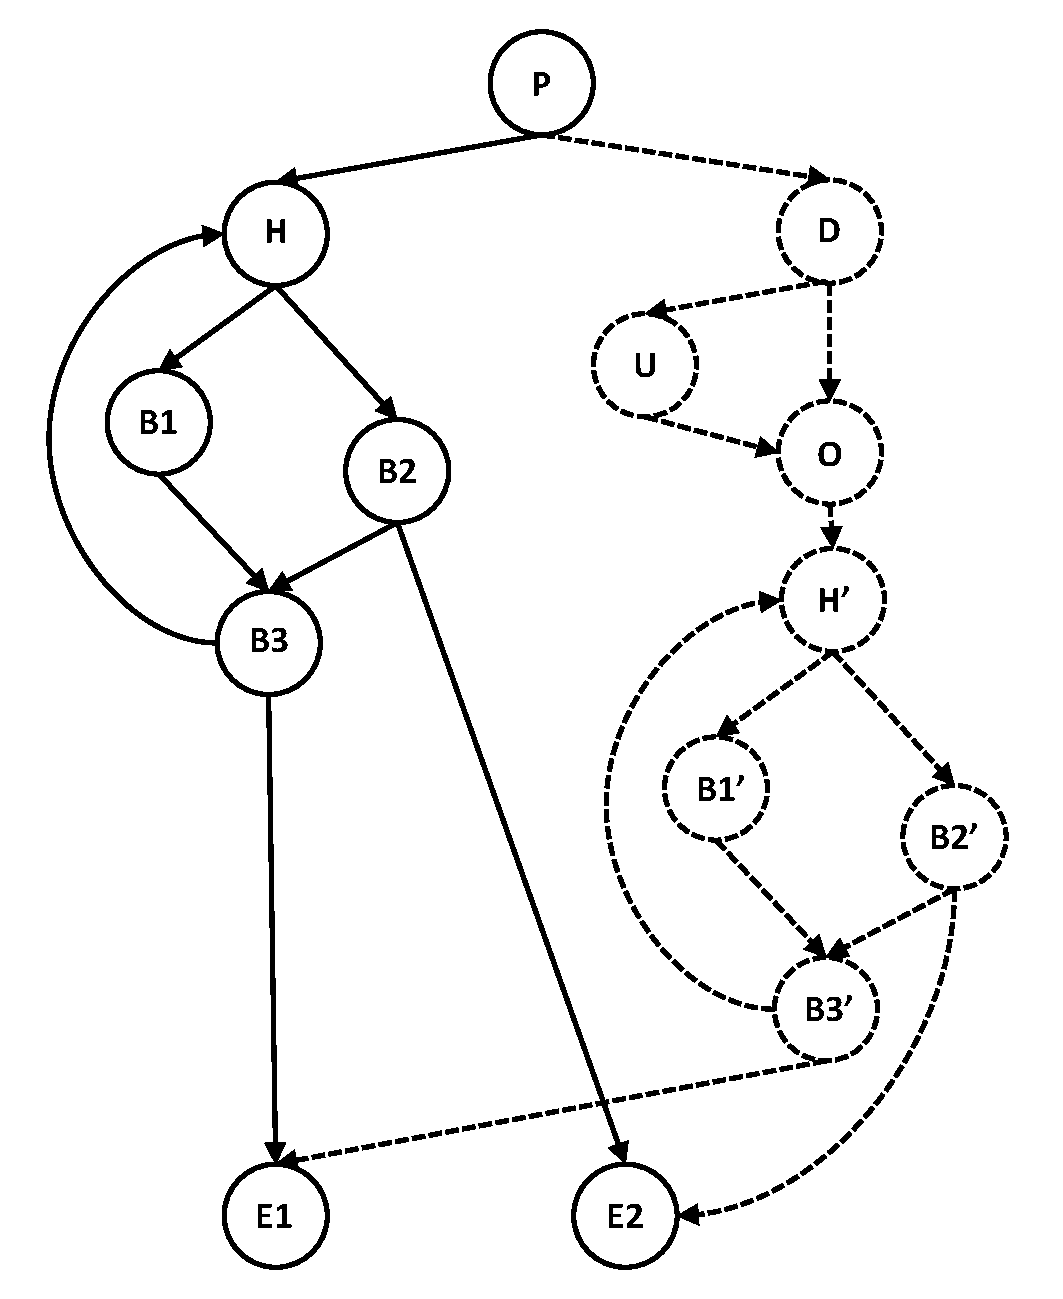
\includegraphics[width=0.7\linewidth]{figures/CL-I}
%\caption{Cross-loop Instrumentation}
%\label{fig:CL-I}
%\end{figure}

Recording values returned by every source instructions would lead to 
huge runtime time. To lower the overhead,
we use random sampling to reduce the number of instructions that we
track at run time. Due to the repetitive nature of performance bugs,
we will still be able to recognize redundant 
computation as long as the sampling rate is not too sparse (we will evaluate
this in Section \ref{sec:6_experiment}). 
Our sampling scheme requires almost no changes to our redundancy 
identification algorithm discussed in Section \ref{sec:6_cal}.


%Another observation, which can also be demonstrated by examples shown in Figure~\ref{fig:Mozilla477564} and Figure~\ref{fig:Apache34464}, 
%is that two consecutive loop instances are good targets to compare.

%There are two possible reasons for cross-iteration redundancy. 
%The first one is loop-invariant computation, which can be identified statically, 
%and it is the target for traditional compiler optimization. 
%The second one is repetitive processed elements, like GCC\#27733 shown in Figure~\ref{fig:GCC27733}. 
%When processed elements are repetitive, the computation conducted by different iterations is exactly the same. 
%If we compare a pair of iterations, we may fail to observe redundancy. 
%For cross-iteration redundancy, we randomly sample iterations, 
%and compare distinct computation number with the total number of sampled iterations. 

\paragraph{Cross-iteration redundancy analysis}
Our high-level sampling strategy is straightforward:
randomly decide at the
beginning of every iteration whether to track the values returned by
source instructions in this iteration.

The implementation is similar with previous sampling work 
\citep{liblit03,liblit05}.
Specifically, we create a clone of the original
loop iteration code, including functions called by the loop directly or
indirectly, and insert value-recording instructions along the
cloned copy. 
We then insert a code snippet that conducts random decision to
the beginning of a loop iteration. 
Two variables \texttt{CurrentID}, which is initialized as 0, 
and \texttt{NextSampleID}, which is initialized by a random integer, 
are maintained
in this code snippet. \texttt{CurrentID} is increased by 1
for each iteration. When it matches \texttt{NextSampleID}, the control
flow jumps to the value-recording clone of the loop iteration and the 
\texttt{NextSampleID} is increased by a random value. Different sampling
sparsity setting will determine the range from which the random value is
generated.

%\begin{figure}
%\center
%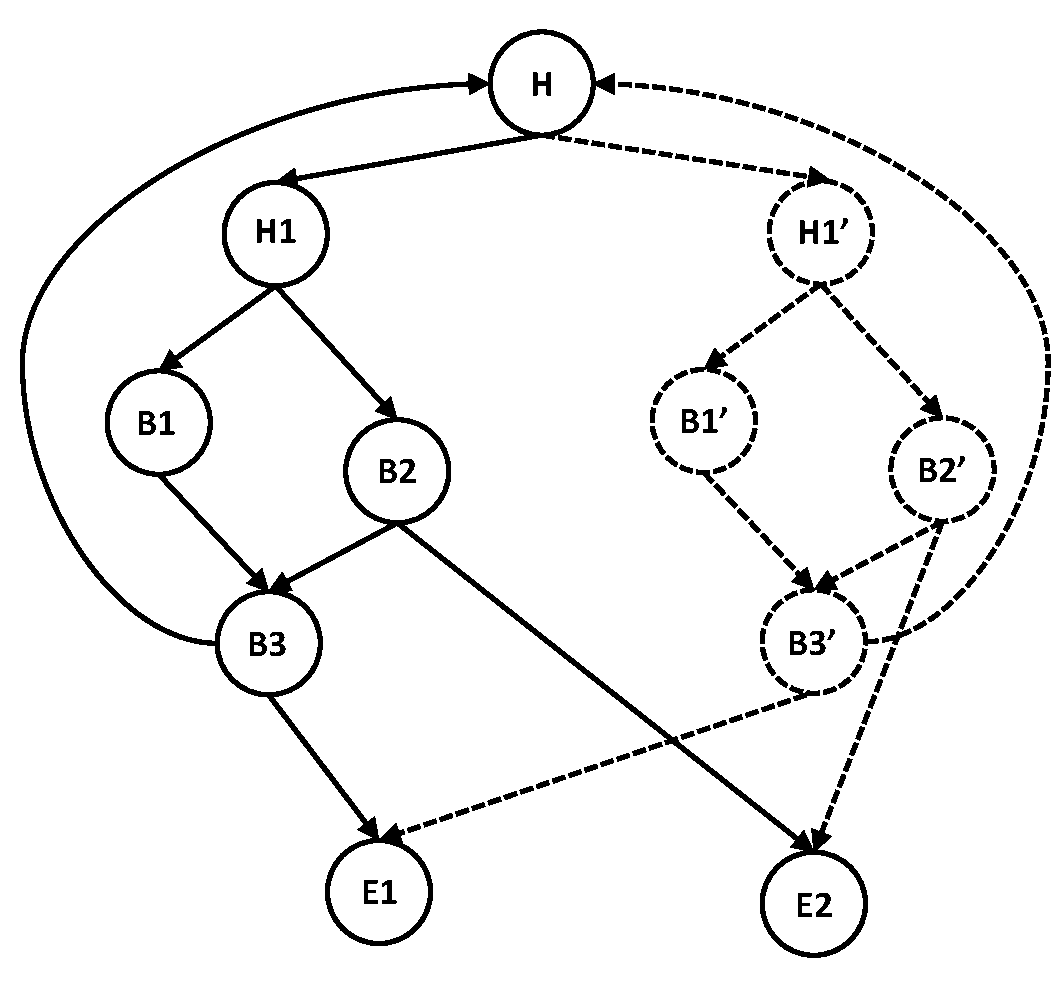
\includegraphics[width=0.7\linewidth]{figures/CI-I}
%\caption{Cross-iteration Instrumentation}
%\label{fig:CI-I}
%\end{figure}

\paragraph{Cross-loop redundancy analysis} 
At high level, we randomly decide at the beginning
of every loop instance whether to track values for this instance. 
Since we will need to compare two consecutive loop
instances for redundancy, once we decide to sample one loop instance, we will
make sure to sample the immediately next loop instance too.

The implementation is similar with that for cross-iteration redundancy analysis.
The only difference includes: (1) clone is made for the whole loop and the
sampling control
is done in the pre-header of the loops; (2)
sampling is conducted when \texttt{CurrentID} equals either
\texttt{NextSampleID} or \texttt{NextSampleID}$+1$, with \texttt{NextSampleID}
increased by a random value in the latter case.

%TODO
%For each monitored memmove or memcpy instruction, 
%we record its ID, the length of accessed memory, 
%and the content of the accessed memory. 



\paragraph{Handling recursive functions}
We also conduct sampling to our redundancy analysis for recursive functions.
For a recursive function, we first create an instrumented clone copy of 
the whole function body.
We then add a sampling-control code snippet at the entry point of the function,
where \texttt{CurrentID} and \texttt{NextSampleID} are maintained to decide
whether to execute the original function body or the instrumented 
value-recording clone copy.
We also create clones for all the callee functions of the recursive function
under study, so that the sampling decision can be correctly conducted
throughout the call chain.

\subsubsection{Static analysis for performance optimization}
\label{sec:6_perf}

We conduct a series of static analysis to reduce the number of instructions we 
need to monitor. 

First, we identify and avoid monitoring memory reads whose return values can be 
statically proved to
not change throughout one loop instance (i.e., for cross-iteration
redundancy analysis) or multiple loop instances (i.e., for cross-loop redundancy
analysis). Since we implement \Tool at LLVM byte-code level, a major part of this
analysis is already done by LLVM, which lifts loop-invariant memory
accesses out of loops. The only extra analysis we did is to 
prune memory reads whose reading address is loop invariant, and there are no writes 
inside the loop which are possibly conducted on the same address. 
For example, the read address of \texttt{aNode.localName} and \texttt{aNode.namespaceURI}
in Figure~\ref{fig:Mozilla347306} is loop-invariant, and there are no write conducted 
on the same address. 
We do not need to record these two memory reads during cross-iteration redundancy analysis. 
%It is easy to lift read from local variable outside the loop. 
%Compiler is conservative to move read, which may cause exception, outside the loop.
%I think this part of analysis is to prune memory read which is invariant, but unsafe to be moved out by compiler. 
%llvm is very conservative to move memory read from array/structure/global variable/heap variable
%outside the loop.
%what we do is if the read address is loop invariant, and there are no other write possibly 
%write to the same place, we will not record the memory read.

%TODO: Linhai, I don't understand your original writing. Pls rephrase, and provide
%an toy example.
%For each monitored memory read, we use loop-invariant analysis to identify 
%whether the read address is loop-invariant. 
%If the address is invariant, and there are no memory writes whose addresses 
%may/must alias to the read address, we will not instrument the memory read.

%ANSWER:
%while(i=lower[j]; a[i]<100 & i<upper[j]; i++); 
%The memory read upper[j] is conducted in each iteration.
%The read address upper+j is loop-invariant. If there is not write to the same
%address, the read is also loop-invariant, and we do not need to record the memory read.
%we conduct alias analysis, and analysis whether there are memory writes, whose
%address may/must alias to the read address. 

Second, we identify and avoid monitoring some memory reads whose return values 
can be statically proved to be different throughout one loop instance in 
cross-iteration redundancy analysis.
Specifically, for read on loop induction variable, such as i for loop at line 11 of Figure~\ref{fig:Apache34464}, 
%Specifically, reading of loop induction 
%variables, such as XXX, are always identified as source instructions in % variable i for loop at line 12
%cross-iteration redundancy analysis; 
we also know for sure that their return
values are different in different iterations. 
If source instructions include read on loop induction variables, we know that 
there could not be cross-iteration redundancy. 
We use scalar evolution analysis
provided by LLVM to identify induction variables and avoid tracking their
values.
%induction variables are not alwayes identified as source instructions.
%it could be possible that side-effect instructions do not depend on induction variables.
%for example, side-effect instruction may only depend on array content, and array index 
%will not be source instructions

%TODO: Linhai, I find it hard to believe that consider "there will not be
%cross-iteration redundancy simply because induction variable is in the 
%dependent set. Really? The input workload itself could be repititive, and hence
%could still deserve monitoring, right? 
%


%ANSWER: this is true according to how we calculate cross-iteration redundancy.
%We only consider iteration from the same loop instance.
%induction variable will be changed in each iteration by a fix constant, so
%the value of induction variable will be different from each other in each iteration of the same loop instance. 
%The case you mention is 
%for(i=0; i < 10; i ++) {
%  c = A[i]; 
%   ...   // all other computation only depend on c        
% }
%Our dependence analysis will report the memory read A[i] as dependent value, not i.
%If the content of A is repetitive, we will identify cross-iteration redundancy.
 
%For cross-iteration instrumentation, we use scalar evolution analysis to identify 
%whether there are induction variables in the dependent value set. 
%A induction variable will be increased or decreased by a fix amount in each loop iteration. 
%If there are induction variable inside the dependent value set, 
%we know that there will not be cross-iteration redundancy. 


Third, sometimes we only record the memory-address range of a sequence of memory
read, instead of the value returned by every read, in cross-loop redundancy
analysis. 
The loop at line 11 in Figure~\ref{fig:Apache34464} shows an example.
The content of array \texttt{source} is not heavily modified
throughout the outer-loop, which starts 
at line 30 in the Figure~\ref{fig:Apache34464}.
%We do not have the static analysis to prove the content of array does not change.
%for source[i] for the loop at line 12, we only need to record source, initial value of i and final value of i. 
%TODO
%Do you really do analysis to prove that the source array is not changed?
%ANSWER
%Shan, I do not have invariant analysis to prove the the source array is not changed.
%I remove that part of writing in the last version I sent to you. 
%It is very difficult to implement the invariant analysis.
%I plan to discuss this in limitation part of this section, and say that this could bring false positives.
%There are reasons why I feel it is too difficult to implement the invariant analysis:
%1. it is difficult to find the range (the outer loop) to apply the analysis.
%assume we have loopA, loopB and loopC. loopA contains loopB, and loopB contains loopC. 
%we are analyzing loopC. It could be possible that loopB only execute 1 or 2 iterations, and loopA is the real outer loop
%2. It is very difficult to prove that there is no other loop inside the outer loop which does not write to the same array.
%There could be cases like:
% for(i = 0; i < 10; i++)
%   func(&(A[i]));
% func will write to its parameter.
Therefore, to check whether different inner loop instances read similar
sequence of array data, we only need to record the starting and 
ending array index touched by each inner loop, significantly reduce the 
monitoring overhead. To accomplish this optimization, we again leverage
the scalar evolution analysis provided by LLVM. The scalar evolution analysis
tells us whether the address of a memory read instruction
is a loop induction variable. For example, the address for memory read \texttt{source[i]} is added by one in each loop iteration,
so it is a loop induction variable. 
From the scalar evolution analysis, we know that the starting address is \texttt{source} plus the initial value of \texttt{i}, and the ending address
is source plus the ending value of \texttt{i}.  
%TODO Linhai, I don't understand your original text. The address is 
%source+i; loop induction variable is i. What do you mean by "the read address
%is an induction varaible"? Please rewrite.

%ANSWER
%Shan, both source + i and i are induction variables, becasue both of them 
%will be added by 1 in each iteration. The only difference between these two 
%are their initial values.
%For cross-loop redundant bugs, we also rely on scalar evolution analysis to identify whether the read address
%is an induction variable for each monitored read instruction. 


\subsubsection{Fix strategy recommendation}
\label{sec:6_redundant_fix}
As discussed in Section \ref{sec:6_tax_study}, extra analysis is needed to
decide whether batching or memoization should be suggested to fix a 
loop that conducts redundant computation.

For cross-iteration redundancy, batching is often used towards
batching I/O related operations, based on our empirical study. 
Therefore, we treat I/O related redundancy separately.
Specifically, when the only side effect of a loop is I/O operations
and the same statement(s) is executed in every loop iteration, we report this
as I/O related redundancy problem and suggest batching as a potential fix
strategy. 

For cross-loop redundancy, whether to use memoization or batching often
depends on which strategy is cheaper to use. \Tool uses a simple
heuristic. If 
the side effect of each loop instance is to update 
a constant number of memory locations, like the 
buggy loop in Figure~\ref{fig:Mozilla477564} and Figure~\ref{fig:Apache34464}, 
we recommend memoization. Instead, if the side effect is updating 
an sequence of memory locations, with the number of locations increasing
with the workload, memoization is unlikely to help save much computation.

%we xxx
%TODO

%%if side effect of the loop is to define several scalar value used outside the loop, we recommend memoization.
%%if side effect is to write to distinct memory address or conduct system call, 
%%we recommend batch



\section{Evaluation}
\label{sec:experiment}

\subsection{Methodology}
\label{sec:result_meth}
%Please discuss the potential usage scenarios of \Tool
%How you will use it together with other tools 


\begin{table}
  \centering
  \scriptsize
  \newcommand{\Yes}[1]{\checkmark{}$_#1$}
  \newcommand{\No}[0]{-}
  \begin{tabular}{lcccc}
    \toprule
                         &      	   &                        & {\bf Root}   &          \\
   {\bf BugID}           &  {\bf KLOC}     &  {\bf P. L.}           & {\bf Cause}  & {\bf Fix}\\
   \midrule
   Mozilla347306         & 88              & C                      &  0*1?        & C     \\
   Mozilla416628         & 105             & C                      &  0*1?        & C     \\
   Mozilla490742         & N/A             & JS                     &  C-I         & B       \\
   Mozilla35294          & N/A             & C++                    &  C-L         & B        \\ 
   Mozilla477564         & N/A             & JS                     &  C-L         & M       \\
   \midrule 
   MySQL27287            & 995             & C++                    &  0*1?,C-L        & C     \\
   MySQL15811            & 1127            & C++                    &  C-L         & M \\ 
   \midrule    
   Apache32546           & N/A             & Java                   &  C-I         & B  \\
   Apache37184           & N/A             & Java                   &  C-I         & M  \\
   Apache29742           & N/A             & Java                   &  C-L         & B \\ 
   Apache34464           & N/A             & Java                   &  C-L         & M  \\
   Apache47223           & N/A             & Java                   &  C-L         & B \\
   \midrule
   GCC46401              & 5521            & C                      &  [0$|$1]*    & S   \\
   GCC1687               & 2099            & C                      &  C-I         & M \\
   GCC27733              & 3217            & C                      &  C-I         & M \\
   GCC8805               & 2538            & C                      &  C-L         & B\\
   GCC21430              & 3844            & C                      &  C-L         & M \\
   GCC12322              & 2341            & C                      &  1*          & S\\
\bottomrule
   \end{tabular}
  %\nocaptionrule
  \caption{Benchmark information.
  (N/A: we skip the size of benchmarks that are extracted from real-world applications.
  Root cause ``C-I'' is short for cross-iteration redundancy.
  Root cause ``C-L'' is short for cross-loop redundancy.
  C, B, M, and S represent different fix strategies, as discussed in
  Table \ref{tab:root}.
  ) 
 }
  \label{tab:benchmarks}
\end{table}

\paragraph{Implementation and Platform}
We implement \Tool in LLVM-3.4.2 \citep{llvm}, and conduct our
%Our implementation consists of 17654 lines of C++ code, 
%with 4748 for instrumenter, 674 for resultless analysis, 
%5802 for redundancy analysis, 
%and the remaining 6430 for common utilities. 
experiments on a i7-960 machine, with Linux 3.11 kernel. 

\paragraph{Benchmarks}
We use 18 out of the 45 bugs listed in Table \ref{tab:root} as our 
evaluation benchmarks. Among these 18, seven are extracted from Java or JavaScript
programs and re-implemented in C++, as \Tool currently only handles C/C++
programs; one is extracted from a very old version of Mozilla.
%These 18 bugs include all the benchmarks used in the recent
%statistical performance debugging work~\cite{SongOOPSLA2014}.
The remaining bugs listed in Table \ref{tab:root} are much more difficult to
use as benchmarks, 
either because they depend on special hardware/software environment
or because they involve too complex data structures to extract. 
Overall, these 18 bugs cover a wide variety of performance root causes, as 
shown in Table~\ref{tab:benchmarks}. 

\paragraph{Metrics}
Our experiments are designed to evaluate \Tool from three main aspects:
\begin{itemize}
\item Coverage. Given our benchmark suite that covers a wide variety
of real-world root causes, can \Tool identify all those root causes?
\vspace{-0.05in}

\item Accuracy. 
When analyzing non-buggy loops, will \Tool generate any false positives?
\vspace{-0.05in}

\item Performance. 
What is the run-time overhead of \Tool?
\end{itemize}

\paragraph{Evaluation settings}
The imagined usage scenario of \Tool is that one will apply \Tool to identify
detailed root causes and provide fix-strategy suggestion for a small number of
suspicious loops that are most correlated with the specific performance problem.

Our evaluation uses existing statistical performance diagnosis
tool \citep{SongOOPSLA2014} to process a performance problem and identify 
one or a few suspicious loops for \Tool to analyze.
For 14 out of the 18 benchmarks, statistical performance debugging identifies the
real root-cause loop as the top ranked suspicious loop. For the remaining
benchmarks, the real root-cause loops are ranked number 2, 2, 4, and 10.
%Overall, we believe future tools can accurately identify the most one or a couple
%of suspicious loops.

\begin{table}
  \centering
  \scriptsize
  \newcommand{\Yes}[0]{\checkmark}
  \newcommand{\No}[0]{-}
  \begin{tabular}{lcc}
    \toprule
                            	&  {\bf Reported}             &{\bf Fix }                     \\
   {\bf BugID}                  &  {\bf Root Cause}           &{\bf Suggestion}             \\
   \midrule
   Mozilla347306                & \Yes                        & \Yes                                          \\
   Mozilla416628                & \Yes                        & \Yes                                         \\
   Mozilla490742$_a$            & \Yes                        & \Yes                                             \\
   Mozilla35294$_a$             & \Yes                          & \Yes                                              \\ 
   Mozilla477564$_a$            & \Yes                          & \Yes                                            \\
   \midrule 
   MySQL27287                   & \Yes                          & \ding{55}                                         \\
   MySQL15811                   & \Yes                          & \Yes                                      \\ 
   \midrule    
   Apache32546                  & \Yes                          & \Yes                                      \\
   Apache37184$_a$              & \Yes                          & \Yes                                        \\
   Apache29742$_a$              & \Yes                          & \Yes                                       \\ 
   Apache34464                  & \Yes                          & \Yes                                        \\
   Apache47223                  & \Yes                          & \Yes                                       \\
   \midrule
   GCC46401                     & \Yes                     & \Yes                                      \\
   GCC1687                      & \Yes                          & \Yes                                     \\
   GCC27733$_a$                 & \Yes                          & \Yes                                     \\
   GCC8805                      & \Yes                          & \Yes                                  \\
   GCC21430                     & \Yes                          & \Yes                                     \\
   GCC12322                     & \Yes                         & \ding{55}                                   \\
   \bottomrule
   \end{tabular}
  %\nocaptionrule
  \caption{Coverage Results.}
  \label{tab:cover}
\end{table}


To evaluate the coverage, accuracy, and performance of \Tool, we mainly conduct
three sets of evaluation. First, we apply \Tool to the real root-cause loop to
see if \Tool can correctly identify the root-cause category and provide
correct fix-strategy suggestion. Second, we apply
statistical performance debugging \citep{SongOOPSLA2014} to all our benchmarks
and apply \Tool to the top 5 ranked loops\footnote{Some extracted benchmarks
have fewer than 5 loops. We simply apply \Tool to all loops in these cases.}
to see how accurate \Tool is. Third, we evaluate the run-time performance of
applying \Tool to the real root-cause loop. 
 
For all benchmarks we use, real-world
users have provided at least one problem-triggering input in their on-line 
bug bugs. We use these inputs in our run-time analysis.

As discussed in Section \ref{sec:design}, our analysis contains 
several configurable thresholds. In our evaluation,
we use 0.001 as the \textit{resultless rate} threshold for identifying
0*1? loops, 0.01 as the \textit{resultless rate} threshold for identifying 
[0$|$1]* loops, 0.5 as the \textit{cross-loop redundancy rate}, and 
2 as the \textit{cross-iteration redundancy rate} (i.e., 
the number of distinct iterations is less than half of the total iterations).

All the analysis and performance results presented below regarding
cross-loop analysis is obtained using $1/100$ sampling rate; all the
results regarding cross-iteration analysis is obtained using $1/1000$ sampling
rate. We use sparser sampling rate in the latter case, because there tend to
be more loop iterations than loop instances.
All our diagnosis results require only \textbf{one} run under the 
problem-triggering input.

\subsection{Coverage Results}
\label{sec:coverage}
Overall, \Tool provides good diagnosis coverage, as shown in Table~\ref{tab:cover}. 
\Tool identifies the correct root cause for \textbf{all} 18 benchmarks, and 
suggests fix strategies that exactly match what developers took in practice
for 16 out of 18 cases. There are only two cases where \Tool fails to suggest
the fix strategy that developers used. For MySQL27287, the root-cause loop
is both cross-loop redundant and 0*1? inefficient. \Tool suggests both changing
data structures and memoization as fix strategies. In practice, the developers
find a new data structure that can eliminate both root causes.
For GCC12322, \Tool correctly tells that the loop under study
does not contain any form of inefficiency and produce results in every 
iteration, and hence fails to suggest any fix strategy. In practice, GCC
developers decide to skip the loop, which will cause some programs compiled by
GCC
to be less performance-optimal than before. However, GCC developers feel
that it is worthwhile considering the performance impact of the original loop
to the GCC compilation process.
Providing this type of
fix strategy suggestion goes beyond the capability of \Tool.

\subsection{Accuracy Results}
\label{sec:result_acc}

\begin{table}
  \centering
  \scriptsize
  \newcommand{\Yes}[0]{\checkmark}
  \newcommand{\No}[0]{-}
  \begin{tabular}{lcccccc}
    \toprule
   {\bf BugID}           &  {\bf 0*1?}          &  {\bf [0$|$1]*}             &{\bf C-I$_b$}            &{\bf C-I$_m$}          &   {\bf C-L}     & {\bf Total}  \\
   \midrule
   Mozilla347306         &   -                  & -                           & -                       & -                     &   -             & -\\
   Mozilla416628         &   -                  & -                           & -                       & -                     &   -             & -\\
   Mozilla490742$_a$     &   -                  & -                           & -                       & -                     &   -             & -\\
   Mozilla35294$_a$      &   -                  & -                           & -                       & -                     &   -             & -\\ 
   Mozilla477564$_a$     &   -                  & -                           & -                       & -                     &   -             & -\\
   \midrule 
   MySQL27287            &   -                  & 0$_1$                       & -                       & -                     &   -             & 0$_1$\\
   MySQL15811            &   -                  & -                           & -                       & -                     &   -             & -\\ 
   \midrule    
   Apache32546           &   -                  & -                           & -                       & -                     &   -             & -\\
   Apache37184$_a$       &   -                  & -                           & -                       & -                     &   -             & -\\
   Apache29742$_a$       &   -                  & -                           & -                       & -                     &   -             & -\\ 
   Apache34464           &   -                  & -                           & -                       & -                     &   -             & -\\
   Apache47223           &   -                  & -                           & -                       & -                     &   -             & -\\
   \midrule
   GCC46401              &   -                  & 0$_1$                       & -                       & -                     &   -             & 0$_1$\\
   GCC1687               &   -                  & -                           & -                       & -                     &   -             & -\\
   GCC27733$_a$          &   -                  & -                           & -                       & -                     &   -             & - \\
   GCC8805               &   -                  & 0$_2$                       & -                       & -                     &   -             & 0$_2$\\
   GCC21430              &   0$_1$              & 0$_3$                       & -                       & 0$_1$                 &   0$_1$         & 0$_6$\\
   GCC12322              &   0$_1$              & 0$_1$                       & -                       & 0$_1$                 &   0$_1$         & 0$_4$\\
\bottomrule
   \end{tabular}
  %\nocaptionrule
  \caption{False positives of \Tool, when applying to top 5 loops reported by 
    statistical performance diagnosis for each benchmark. `-' represents zero false positive.
    Other cells report real false positives and benign false positives, which is in the
    subscript.
}
  \label{tab:top5}
\end{table}

As shown in Table \ref{tab:top5}, \Tool is accurate, having 0 real
false positive and 14 benign false positives for all the top 5 loops.

Here, benign false positives mean that the \Tool analysis result is true ---
some loops are indeed cross-iteration/loop redundant or indeed producing
results in only a small portion of all the iterations. However, those
problems are \textit{not} fixed by developers in their performance patches. 

There are several reasons for these benign performance problems. 
The main reason is that they are not the main contributor to the 
performance problem perceived by the users. This happens to 12 out of the
14 benign cases. In fact, this is not really a problem for \Tool in 
real usage scenarios, because statistical debugging can accurately
tell that these loops are not top contributors to the performance
problems.
The remaining two cases happen when fixing the 
identified redundant/resultless problems
are very difficult and hence developers decide not to fix them.

The accuracy of \Tool benefits from its run-time analysis.
For example, 4 benchmarks contain loops that only generate side-effect
in the last iteration among their top 5 suspicious loops. However,
these loops are actually not inefficient because the portion of
resultless iterations is small. 

The good accuracy of \Tool can actually help improving the accuracy of
identifying which loop is the root cause loop.
For example, the real root-cause loop of Apache34464 and GCC 46401 both
rank number two by the statistical performance diagnosis tool.
\Tool can tell that the number one loops in both cases do not contain
any form of inefficiency, resultless or redundancy. This result can
potentially used to improve the accuracy of identifying root cause loops.


\subsection{Performance}
\label{sec:result_perf}

\begin{table}
  \centering
  \scriptsize
  \newcommand{\Yes}[1]{\checkmark{}$_#1$}
  \newcommand{\No}[0]{-}
  \begin{tabular}{lccccc}
    \toprule
	    & \multicolumn{3}{c}{\Tool} & \multicolumn{2}{c}{w/o optimization} \\
     \cmidrule(lr){2-4}
     \cmidrule(lr){5-6}
     {\bf BugID}  & {\bf Resultless}  &  {\bf C-L R. } & {\bf C-I R. }  & {\bf C-L R.}  & {\bf C-I R. } \\
    \midrule
    Mozilla347306 &  1.07\%           &  22.40\%       &  10.17\%       & 304.37{\bf X} & 468.74{\bf X} \\ 
    Mozilla416628 &  0.80\%           &  4.10\%        &  2.99\%        & 567.51{\bf X} & 85.6{\bf X} \\
    \midrule
     MySQL27287   & $\sim$0           &   1.66\%       &   -            & 109.55{\bf X} & 352.07{\bf X} \\
     MySQL15811   &  -                &   0.03\%       &   -            & 227.04{\bf X} & 424.44{\bf X} \\
    \midrule
      GCC46401    & 3.12\%         & 3.80\%            &  5.95\%        & 21.07{\bf X}  & 38.44{\bf X}\\ 
      GCC1687     & -              & /                 &  $\sim$0       &   /           & 142.29{\bf X} \\
      GCC27733$_a$    & $\sim$0        & /                 &  4.73\%        &   /           & 17.41{\bf X}     \\
      GCC8805     & -              & $\sim$0           & $\sim$0        & 2.22{\bf X}   &  3.52{\bf X}\\
      GCC21430    & -              & 5.46\%            &   0.69\%       & 107.20{\bf X} & 159.89{\bf X} \\
      GCC12322    & -              & 1.75\%            &  $\sim$0       & 21.07{\bf X}  & 38.44{\bf X} \\
   \bottomrule
   \end{tabular}
  %\nocaptionrule
  \caption{Run-time overhead of applying \Tool to the buggy loop, with and
    without optimizations. 
    Only results from non-extracted benchmarks are shown. 
  -: static analysis can figure out the results and hence no dynamic analysis is conducted.
  /: not applicable. }
  \label{tab:performance}
\end{table}




As shown in Table \ref{tab:performance}, 
the performance of \Tool is good. The overhead is consistently under or around 5\% 
except for one benchmark, Mozilla347306. We believe \Tool is promising for potential production
run usage. Of course, if we apply \Tool to multiple loops simultaneously,
the overhead will be higher. However, the current results are obtained by running the
program only \textbf{once} under the problem-triggering workload. The sampling nature
of \Tool will allow us to keep the overhead low at the exchange of running the program for
a couple of more times, if needed.

As we can also see from the table, our performance optimization discussed in 
Section \ref{sec:inst} and \ref{sec:perf} has contributed
a lot to the good performance of \Tool.

Without sampling, while still applying our static optimization, our redundancy
analysis would lead to over 100X slowdown for five benchmarks.

The buggy loops of MySQL\#27287 and MySQL\#15811 access arrays. 
After changing to tracking the initial and ending memory-access addresses
of the array, instead of the content of the whole array accesses,
the overhead is reduced from 11.77\% to 1.66\% for MySQL\#27287, 
and from 20.46\% to 0.03\% for MySQL\#15811 respectively 
(sampling is conducted consistently here). 

The side-effect of the buggy loop for MySQL15811 is to calculate the length of a string. 
The variable representing the length is an induction variable. 
The side-effect of the buggy loop for MySQL27287 is to calculate the index of a searched target, 
and the variable representing the index is also an induction variable. 
We can reply on static analysis to figure out that these two loops are not cross-iteration redundant.

We also tried sampling with different sampling rates.
For cross-loop redundancy, we also conduct experiments under sampling rate 1
out of 1000. 
Both run-time overhead and collected sample will be reduced. Mozilla347306 
is still the benchmark with largest overhead, but the overhead is reduced to 0.49\%. For two benchmarks, GCC8805 and GCC12322, we cannot sample 
more than 10 loop instances and hence cannot draw strong conclusion
about their root-cause type. For all other benchmarks, we can 
still have more than 10 loop instances and get exactly the same 
root-cause analysis results presented above.

We also conduct cross-iteration redundant experiment under different sampling rates. When the sampling rate is 1 out of 100, there are two benchmarks, whose runtime overhead is larger than 30\%. The overhead for Mozilla347306 is 59.57\%, 
and the overhead of GCC21430 is 30.65\%. When changing sampling rate to 1
out of 10000, Mozilla347306 has the largest overhead, which is 4.47\%. And mozilla347306 is the only one whose overhead is larger than 2\%. Except for 
GCC12322, all other benchmarks will have more than 100 iterations sampled, under the sample rate is 1 out of 10000. Consequently, the same root-cause
analysis results will be reported for these benchmarks as the ones presented
above.

\section{Conclusion}
\label{sec:con}
Performance diagnosis is time consuming and also critical for 
complicated modern software. \Tool tries to automatically 
pin-point the root cause of
the most common type of real-world performance problems, inefficient loops,
and provide fix-strategy suggestions to developers. It achieves the 
coverage, accuracy, and performance goal of performance diagnosis by leveraging
(1) a comprehensive root-cause taxonomy; (2) a hybrid static-dynamic program
analysis approach; and (3) customized random sampling that is a natural fit for 
performance diagnosis.
Our evaluation shows that \Tool can accurately identify detailed root causes
of real-world inefficient loop problems and provide fix-strategy suggestions. 
Future work can further improve \Tool by providing more detailed fix
suggestions and providing more information to help diagnose and fix
1* loops.

